\chapter{Implementation}
\label{ch:implementation}
In this chapter we go over the details of the software implementations we created during our study. To this end, we introduce the use-case and context of the model project. Afterwards, we summarize the architecture details of the original implementation. Finally, we introduce the three implementation variants we created and explain our design decisions.  

\section{Chauffeur Service}
As a basis for our case study we used an application called DSW-FD (Dispositions-software-Fahrdienst). DSW-FD is used to schedule chauffeur rides for a German federal agency. The application provides a rich user interface with views for managing chauffeur jobs as well as chauffeur drivers. Clients which need a chauffeur ride can call a separate hotline where a handler creates a new chauffeur job. This job is then sent to DSW-FD where it appears in the overview of jobs and can then be processed by a dispatcher.

Drivers need to be manually assigned to a job by the dispatcher. To this end, the application provides suggestions for drivers which would be free when the job is scheduled and are closest to the job's departure point. Furthermore, the app provides functionality to group together different jobs so that they may be handled by a single driver, determine the return destination for the driver after they finished the job, as well as marking a job as being handled by a pool of drivers.

The application also provides features to directly interact with drivers, such as broadcasting messages to all drivers, reminding a driver to take their mandatory break, and directly calling a driver.

\section{Current Implementation}
The current Implementation is realized using a classic frontend-backend architecture. The backend is implemented using the Java web framework Spring\footnote{\url{https://spring.io/}}. It provides a SOAP web server on which new jobs are submitted from another service. Data is persisted in a MSSQL database. The backend also provides Multiple REST APIs and an OData API for communication with the frontend. Furthermore, the backend has to interact with Firebase to trigger push notifications on smartphone devices.

The system provides two frontends, an android application, which is used by the chauffeur drivers to receive jobs and communication from headquarters, and a web client which is used by handlers to manage jobs and drivers. The web client is implemented using OpenUI5\footnote{\url{https://openui5.org/}}. OpenUI5 is a frontend framework published by SAP, it is intended for development of enterprise applications which follow SAP's Fiori design guidelines\footnote{\url{https://experience.sap.com/fiori-design/}}. All APIs of the backend require authentication. To this end the frontend has to authenticate with a Keycloak\footnote{\url{https://www.keycloak.org/}} instance using OpenID Connect (OIDC). An overview of the system architecture is provided in \Cref{fig:dswfd-architecture}.

\begin{figure}[ht]
    \centering
    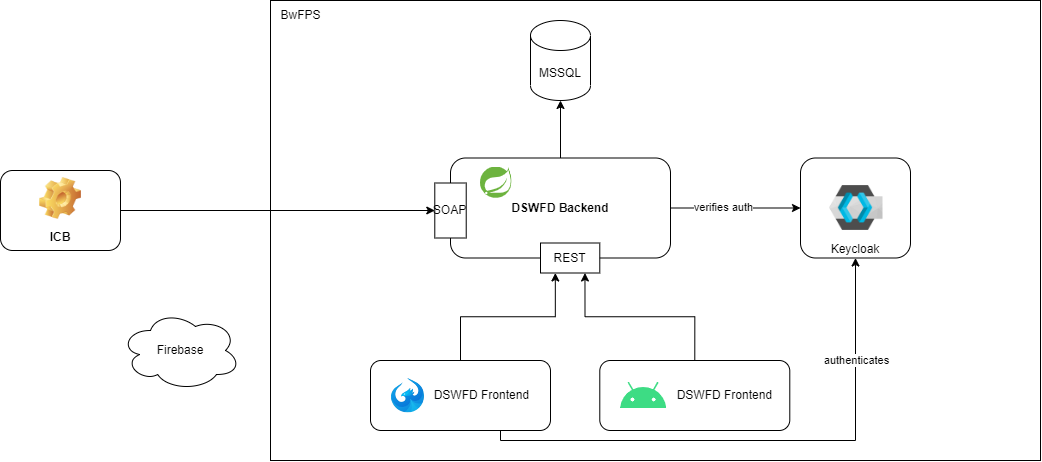
\includegraphics[width=.8\linewidth]{assets/dswfd-architecture}
    \caption{Architecture overview of the original implementation}
    \label{fig:dswfd-architecture}
\end{figure}

\section{SvelteKit Implementation}
Our study focused on the core of DSW-FD's system landscape, comprised of the Spring backend and the OpenUI5 web frontend. We experimented with two different implementations. One where SvelteKit replaces both the backend and frontend, and one where SvelteKit only replaces the frontend. Both our implementations had to communicate with the Keycloak service to authenticate. The full stack implementation also had to interact with the MSSQL database. As to focus on the most relevant parts, APIs for the android application, Firebase communication, and the SOAP API for ICB were not implemented. We also decided to use TypeScript instead of regular JavaScript. This provided a better developer experience with little extra overhead. Because SvelteKit can infer types for most of its internal functionality, extra types had to be only defined for external APIs.

We focused our implementation on a subset of features required to manage chauffeur jobs. To this end we implemented three pages: the overview page that shows all currently relevant chauffeur jobs (\Cref{fig:current-overview-auftrag}), the detail page for chauffeur jobs (\Cref{fig:current-details-auftrag}), and a view that is used to create new (internal) chauffeur jobs.

\begin{figure}
    \centering
    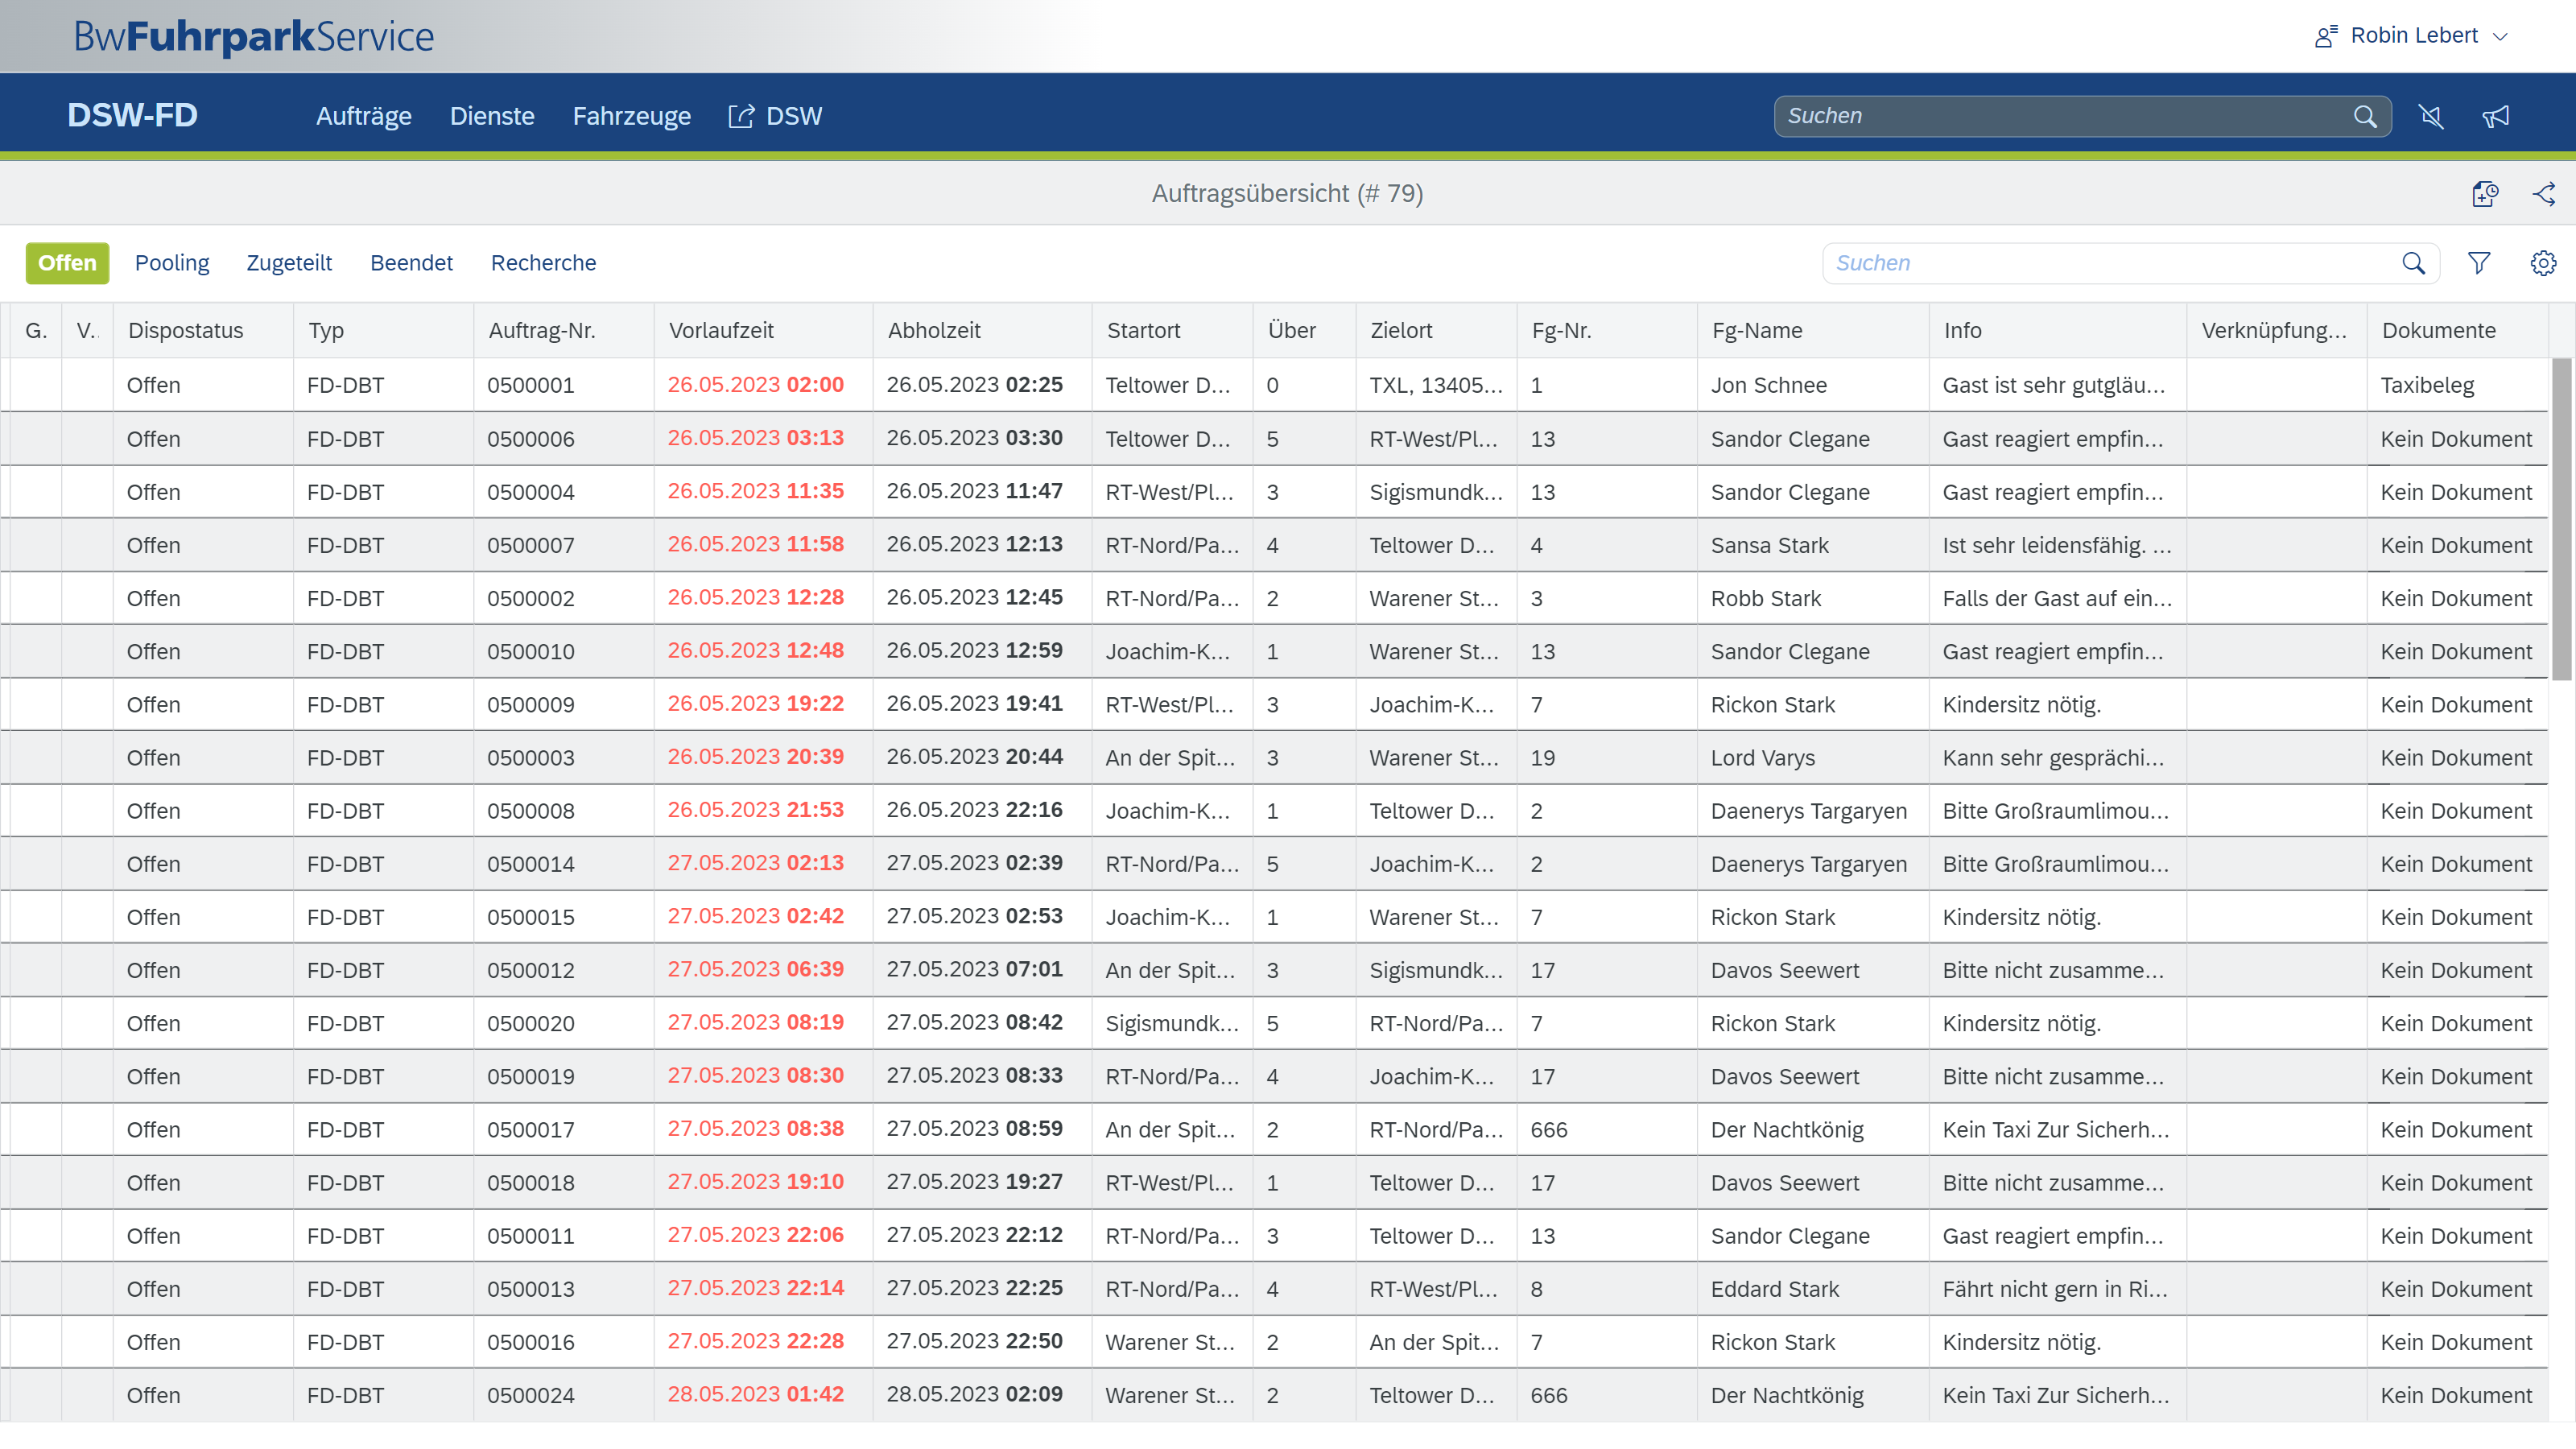
\includegraphics[width=\linewidth]{assets/current-auftrag-overview}
    \caption{Overview of chauffeur jobs in current implementation filled with dummy data.}
    \label{fig:current-overview-auftrag}
\end{figure}

\begin{figure}
    \centering
    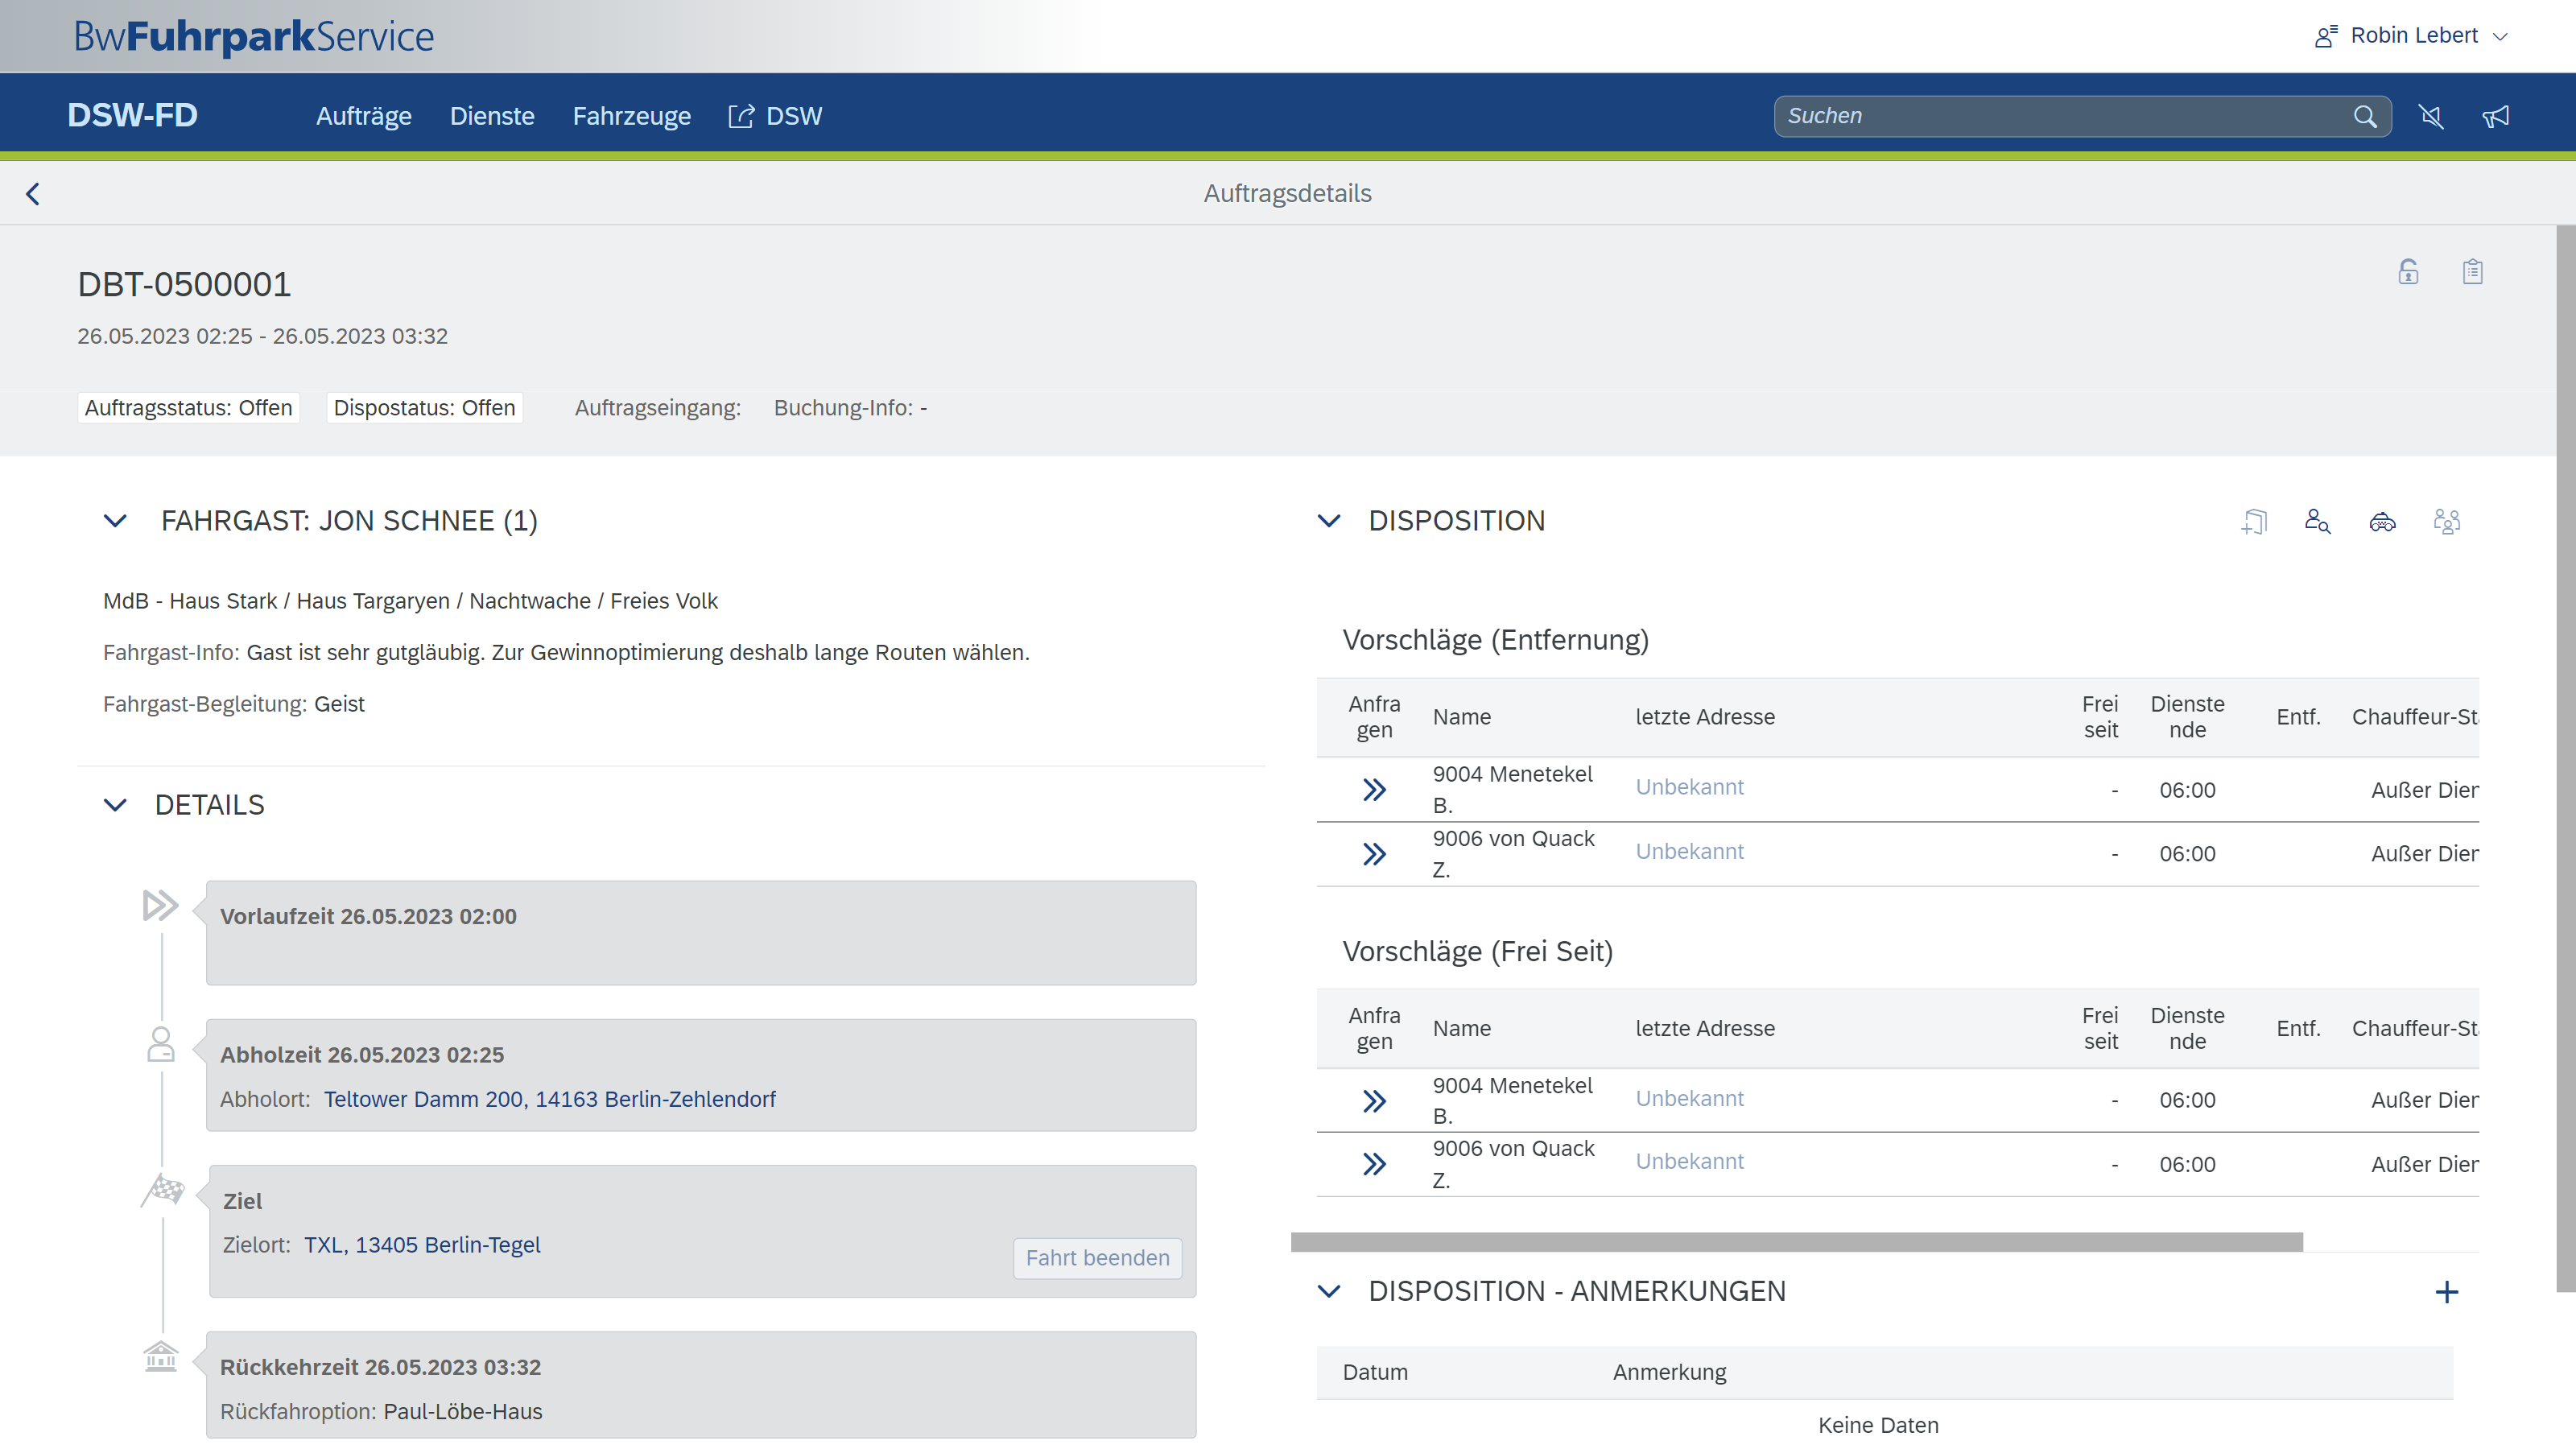
\includegraphics[width=\linewidth]{assets/current-auftrag-details}
    \caption{Chauffeur job details view in current implementation for a dummy job.}
    \label{fig:current-details-auftrag}
\end{figure}


\subsection{Full Stack Implementation}
Our first approach was the full stack implementation. This implementation has to replace the UI5 frontend as well as the Spring backend (\Cref{fig:dswfd-architecture-fullstack}). To this end, business logic, database communication and API's all had to be implemented in SvelteKit. We used Prisma\footnote{\url{https://www.prisma.io}} for object relational mapping to communicate with the database, because Prisma provides functionality to generate its data model from an existing database using introspection. This allowed us to save time on defining models. 

This implementation makes use of SvelteKit's server load functions (\Cref{sec:sveltekit-loading}). The load function for each page calls a separate service function which queries required data from the database. For posting data to the server we used SvelteKit's recommended mechanism, form actions (\Cref{sec:sveltekit-form-actions}). Form actions send \mintinline{text}{FormData} objects\footnote{\url{https://developer.mozilla.org/en-US/docs/Web/API/FormData}} to the server. These objects hold the raw request data as key-value pairs. To validate the correctness of this data we used Zod\footnote{\url{https://zod.dev/}}. Zod is a schema validation library that can be used to define constraints that a data structure has to satisfy. Furthermore, with the extension \mintinline{text}{zod-form-data}\footnote{\url{https://www.npmjs.com/package/zod-form-data}}, Zod can be used to parse \mintinline{text}{FormData} objects into a given data structure. This overall improved the ergonomics of using SvelteKit's form actions.  

% Business logic could be ported directly from Java to TypeScript, which made it a primarily laborious task. 

\begin{figure}
    \centering
    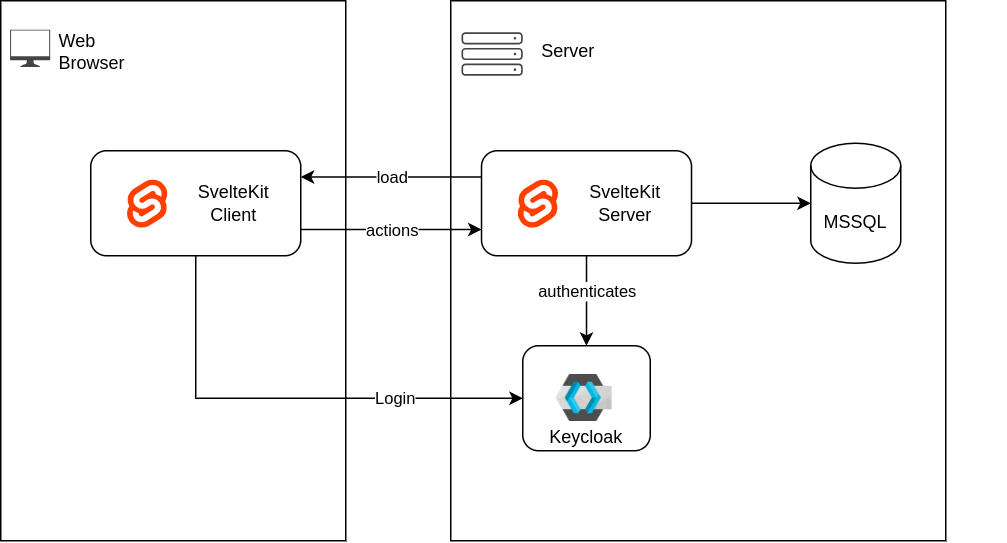
\includegraphics[width=.8\linewidth]{assets/dswfd-architecture-fullstack}
    \caption{Architecture overview of the implementation using SvelteKit as a full stack framework}
    \label{fig:dswfd-architecture-fullstack}
\end{figure}

\subsection{Frontend Implementation}
We also decided to explore an approach where SvelteKit is only used as a frontend. This approach provides more flexibility because backend technology can be chosen individually. Communication to the backend is primarily handled using web APIs. In our use case we decided to reuse the existing Java backend. The backend's REST API could be queried from SvelteKit. As REST APIs are something which can be called from frontend and backend, this approach can make use of SvelteKit's universal load functions (\Cref{sec:sveltekit-loading}). This means that the SvelteKit server is only used during SSR. After the browser has loaded the page, universal load functions are executed client-side. The client then directs its requests directly to the backend instead of sending a request to the SvelteKit server which then requests the data from the backend. Therefore, saving one unnecessary hop. If loss of SSR is acceptable, this approach would also make it possible to run the application as an SPA, forgoing a dedicated SvelteKit server (\Cref{fig:dswfd-architecture-spa}). This can be useful, as it allows for the SvelteKit application to be served as static files from a web directory or similar.

\begin{figure}[ht]
    \centering
    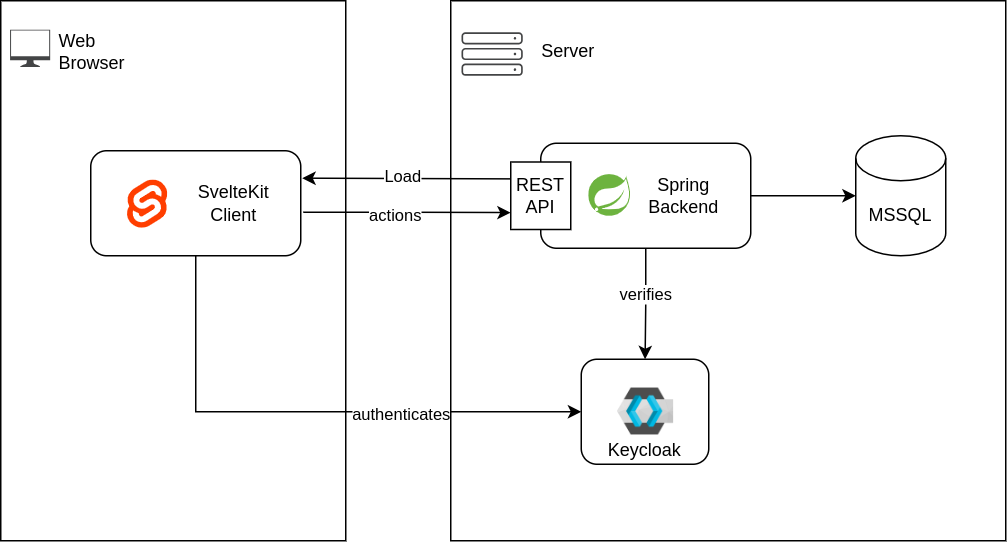
\includegraphics[width=.8\linewidth]{assets/dswfd-architecture-spa}
    \caption{Architecture overview of the implementation using SvelteKit as an SPA framework without a dedicated SvelteKit server.}
    \label{fig:dswfd-architecture-spa}
\end{figure}

\subsection{SPA Implementation}
\label{sec:implementation-redirect}
But this approach has several shortcomings explained in \Cref{sec:evaluation-universal}. Therefore, we further experimented with an implementation that again uses server load functions and server actions. This implementation is very similar to the full stack implementation discussed earlier. But instead of implementing business logic and database access in the SvelteKit server side code, the server side is primarily used as middleware that sends REST requests to the Spring backend \Cref{fig:dswfd-architecture-frontend}.

\begin{figure}[ht]
    \centering
    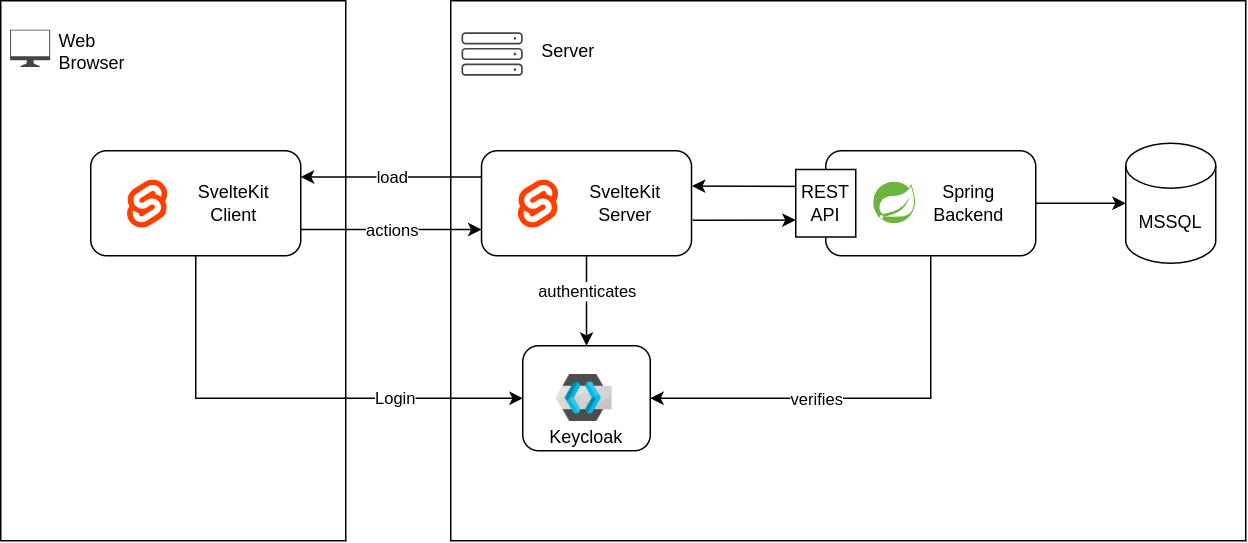
\includegraphics[width=.9\linewidth]{assets/dswfd-architecture-frontend}
    \caption{Architecture overview of the implementation using SvelteKit only for the frontend where the SvelteKit server serves as a middleware to handle communication with the Spring backend.}
    \label{fig:dswfd-architecture-frontend}
\end{figure}

This approach has multiple advantages. It uses much of the built-in functionality of SvelteKit, applications can be progressively enhanced, the client requires fewer dependencies, because functionality such as parsing and validating form data can be handled server side. Furthermore, authentication is simplified, as only the backend needs to communicate with the API. And finally, the outlined problems with fetch in universal load functions is solved, because only the backend uses fetch.


\subsection{UI Considerations}
\label{sec:implementation-ui}
One of the project client's requirements for the original implementation was that the frontend follows the SAP Fiori design guidelines. While not strictly necessary for our study, we decided to adhere to this requirement in our SvelteKit implementations. We hoped to gain insights into how SvelteKit behaves when interacting with UI libraries. The current implementation uses UI5 which has SAP Fiori components built into the framework itself. As it is not possible to use these components outside the framework, we had to use alternatives.   

We first tried to use UI5 Web Components\footnote{\url{https://sap.github.io/ui5-webcomponents/}}. These premade components promise to be a feature rich and framework-agnostic implementation of the Fiori Design Guidelines. In practice, we noticed issues with this approach which will be discussed in \Cref{sec:evaluation-ui-libs}. Therefore, we decided to use SAP Fundamental Styles\footnote{\url{https://sap.github.io/fundamental-styles/}}, a library that provides CSS styles to create Fiori components. We then built a custom UI Component library around these styles. This had the added benefit of providing insights into how Svelte performs for creating UI components.


% Our first approach was to use SAP's UI5 Web components. Web components promise to be a framework-agnostic approach to UI components. But we encountered some problems early on:

% \begin{itemize}
%     \item For now, web components can not be server-side rendered. This is because web components rely on API's which only exist in the browser
%     \item Web Components also require JavaScript (at least until \cite{noauthor_declarative_2023})
%     \item Problems: Layout shifting, flash of unstyled content ("FOUC")
% \end{itemize}
